\documentclass{article}

\usepackage[letterpaper, portrait, margin=1.5in]{geometry}

\usepackage{fancyhdr}
\usepackage{ragged2e}
\usepackage{graphicx}
\usepackage{caption}
\usepackage{amsmath}
\usepackage{rotating}

\usepackage{listings}
\usepackage{color}

\definecolor{dkgreen}{rgb}{0,0.6,0}
\definecolor{gray}{rgb}{0.5,0.5,0.5}
\definecolor{mauve}{rgb}{0.58,0,0.82}

\lstset{frame=tb,
  language=Java,
  aboveskip=3mm,
  belowskip=3mm,
  showstringspaces=false,
  columns=flexible,
  basicstyle={\small\ttfamily},
  numbers=none,
  numberstyle=\tiny\color{gray},
  keywordstyle=\color{blue},
  commentstyle=\color{dkgreen},
  stringstyle=\color{mauve},
  breaklines=true,
  breakatwhitespace=true,
  tabsize=4
}

\setcounter{secnumdepth}{1}

\usepackage{chngcntr}
\counterwithin{figure}{section}

\renewcommand*{\thepage}{C\arabic{page}}

\pagestyle{fancy}
\lhead{ACME Robotics}
\chead{\#8367}
\rhead{\ifcontents Contents \else Week \thesection \fi}

\newif\ifcontents
\contentstrue

\makeatletter
\renewcommand{\@seccntformat}[1]{}
\makeatother
\begin{document}
\subsection{Parts List}
%! Assemble a parts list of orders needed for the next stage of building.
Since the team was planning a lot of revisions for the robot, Jon and Oren put together a parts list for all the parts they would need (figure \ref{fig: Parts list}). It is important that the team stay organized and keep a clear record of all the parts they buy. This makes sure that ACME keeps track of their budget (both how much money they have and how much they have spent), which parts have been ordered and which have not, and which parts they need in the first place. It also helps whoever is ordering the parts to know exactly which parts to buy and where to get them. without doing things like this to keep organized, almost nothing would be done in a timely fashion. To create this list in the first place, ACME had a hardware meeting similar to the previous one to confirm and list all the changes that they wanted to make to the robot. As you can see in image . This ensured that everyone on the team was on the same page about what was changing on the robot, what needed to be bought and built to do so, and to give a basis for a parts list. It is important that all team members are on the same page so that time and resources are not wasted. If someone on the team is spending time and material building a mechanism that the team has decided does not need to be there, then that time and resources have been wasted. Keeping everyone on the same page about what is happening to the robot keeps everything running more efficiently.

\begin{figure}
    \centering
    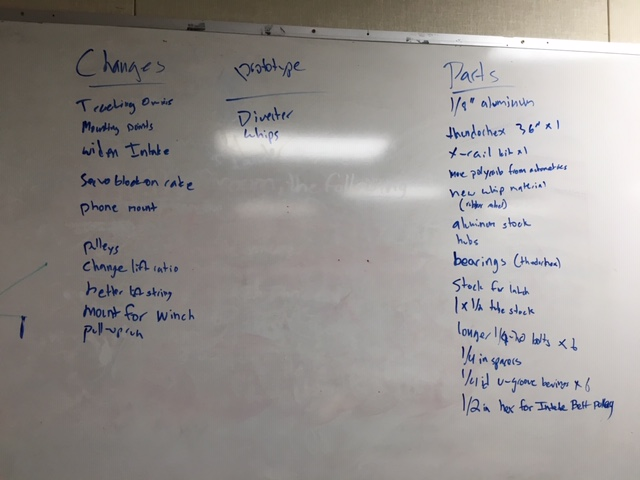
\includegraphics[width=.6 \textwidth]{14_12-03/images/IMG_0422.JPG}
    \caption{The Final Parts List}
    \label{fig: Parts list}
\end{figure}

\end{document}